% arXiv submission - standard article class
% Clean version with proper encoding
% File: lfunction_zeros_2026_clean.tex

\documentclass[11pt, a4paper]{article}
\usepackage[utf8]{inputenc}
\usepackage[T1]{fontenc}
\usepackage{amsmath, amssymb, amsthm}
\usepackage{graphicx}
\usepackage{xcolor}
\usepackage[colorlinks=true, allcolors=blue]{hyperref}
\usepackage{url}
\usepackage{booktabs}
\usepackage[expansion=false]{microtype}
\usepackage{natbib}
\usepackage{xspace}

% Keywords (not defined in article class)
\providecommand{\keywords}[1]{\par\medskip\noindent\textbf{Keywords:} #1}

% Custom commands for text mode
\newcommand{\ie}{i.e.,\xspace}
\newcommand{\eg}{e.g.,\xspace}
\newcommand{\etc}{etc.\xspace}
\newcommand{\SL}{\textsl{SL}}
\newcommand{\GL}{\textsl{GL}}
\newcommand{\GUE}{\textsc{GUE}}
\newcommand{\GOE}{\textsc{GOE}}
\newcommand{\GSE}{\textsc{GSE}}
\newcommand{\Poisson}{\textsc{Poisson}}
\newcommand{\LMFDB}{\texttt{LMFDB}}
\newcommand{\Fp}{\ensuremath{\mathbb{F}_p}}

% Theorem environments
\newtheorem{theorem}{Theorem}
\newtheorem{lemma}[theorem]{Lemma}
\newtheorem{proposition}[theorem]{Proposition}
\newtheorem{corollary}[theorem]{Corollary}
\newtheorem{conjecture}[theorem]{Conjecture}
\newtheorem{remark}[theorem]{Remark}
\newtheorem{example}[theorem]{Example}

\title{The Two-Population Structure of L-Function Zero Spacings: \\ dim=1 to \GUE{}, dim$\geq$2 to \Poisson{} with 6\% Outliers}
\author{Tobias Weiss}
\date{\today}

\begin{document}

\maketitle

\begin{abstract}
We present empirical evidence for a two-population structure in the spacing statistics of L-function zeros for modular forms, revealing a dimension-dependent transition from Gaussian Unitary Ensemble (\GUE{}) to \Poisson{} statistics. Analyzing 63,844 weight-2 newforms from the \LMFDB{} database with 10 lowest zeros each, we find: (1) dim=1 forms (elliptic curves) exhibit \GUE{} statistics with Brody $\beta=1.88$ ($R^2=0.99$ vs \GUE{} reference), (2) dim$\geq$2 forms exhibit near-\Poisson{} statistics with $\beta=0.24$, and (3) within dim$\geq$2, 6\% of forms retain \GUE{} statistics, characterized as low-dimension, small-level forms. Surprisingly, spectral rigidity properties are predictable from scalar metadata (dimension, level, analytic rank) alone with $R^2>0.93$, while Hecke trace features contribute negligible additional signal ($\Delta R^2<0.02$). This suggests that spacing statistics are determined by the form's arithmetic complexity rather than its specific Hecke eigenvalue sequence. Our results refine the Katz-Sarnak philosophy and provide a novel lens on the distribution of L-function zeros.

\keywords{L-function zeros, random matrix theory, modular forms, spacing statistics, Brody ensemble, machine learning}
\end{abstract}

\tableofcontents

\section{Introduction}
\label{sec:introduction}

The distribution of zeros of L-functions has been a central topic in number theory since Riemann's 1859 paper on the zeta function~\cite{riemann1859}. A complementary question, initiated by Hugh Montgomery in 1973~\cite{montgomery1973}, concerns the statistical distribution of zeros. Montgomery discovered that the pair correlation of Riemann zeta zeros matches that of the Gaussian Unitary Ensemble (\GUE{}) from random matrix theory~\cite{montgomery1973,mehta2004}. This led to the Dyson-Montgomery conjecture~\cite{dyson1962,montgomery1973}: the zeros of the Riemann zeta function, and more generally L-functions, are distributed like the eigenvalues of random Hermitian matrices.

The Katz-Sarnak philosophy~\cite{katzsarnak1999} extends this conjecture to families of L-functions, predicting that zero spacing statistics match those of classical random matrix ensembles (\GOE{}, \GUE{}, \GSE{}) based on the symmetry type of the family. For elliptic curves (dimension-1 Galois representations), the \GUE{} ensemble is predicted~\cite{katzsarnak1999} and has been empirically verified~\cite{odlyzko1987}.

However, the behavior of L-functions for higher-dimensional modular forms has received less attention. This paper presents the first large-scale empirical study of zero spacing statistics across all dimensions.

\subsection{Our Contributions}

We make four main contributions:

\begin{enumerate}
\item {\bfseries Two-population structure}: dim=1 forms exhibit \GUE{} statistics ($\beta=1.88$) while dim$\geq$2 forms exhibit near-\Poisson{} statistics ($\beta=0.24$).

\item {\bfseries Continuous transition}: The transition from \GUE{} to \Poisson{} is gradual with dimension: dim=2 has 11.8\% \GUE{} preference, dim=3 has 5.8\%, dim$\geq 4$ has 3-4\%.

\item {\bfseries \GUE{} outliers characterized}: Within dim$\geq$2, 6\% of forms retain \GUE{} statistics. These are systematically low-dimension (mean dim=4.03 vs 6.22), small-level (mean level=2,590 vs 2,792) forms.

\item {\bfseries Predictability from metadata}: Spectral rigidity properties (spacing mean, std, \GUE{} preference) are predictable from scalar metadata alone with $R^2>0.93$. Hecke trace features add negligible value ($\Delta R^2<0.02$).
\end{enumerate}

\section{Background}
\label{sec:background}

\subsection{Modular Forms and L-Functions}

Let $\Gamma = \SL(2, \mathbb{Z})$ be the special linear group over the integers. A modular form of weight $k$ is a holomorphic function $f: \mathbb{H} \to \mathbb{C}$ satisfying the transformation property $(f \mid_k \gamma)(z) = f(z)$ for all $\gamma \in \Gamma$, where $\mathbb{H}$ is the upper half-plane.

To each modular form, one can associate an L-function $L(s, f) = \sum_{n=1}^{\infty} a_n n^{-s}$, where the coefficients $a_n$ are the Hecke eigenvalues.

\subsection{Random Matrix Theory}

The spacing distribution of eigenvalues in random matrix ensembles provides a powerful statistical framework. For nearest-neighbor spacings, the classical ensembles have distinct distributions:

\begin{itemize}
\item {\bfseries \Poisson{}}: Uncorrelated eigenvalues, $P(s) = e^{-s}$
\item {\bfseries \GOE{}}: Orthogonal ensemble, $P(s) \approx (\pi s / 2) e^{-\pi s^2 / 4}$
\item {\bfseries \GUE{}}: Unitary ensemble, $P(s) \approx (32 s^2 / \pi^2) e^{-4 s^2 / \pi}$
\end{itemize}

The Brody ensemble~\cite{brody1981} provides a continuous interpolation between \Poisson{} ($\beta=0$) and \GOE{} ($\beta=1$):
\begin{equation}\label{eq:brody}
P_\beta(s) = c_\beta s^\beta e^{-a_\beta s^{\beta+1}},
\end{equation}
where $c_\beta$ and $a_\beta$ are normalization constants.

\subsection{The Katz-Sarnak Philosophy}

Katz and Sarnak~\cite{katzsarnak1999} conjecture that the spacing statistics of zeros of L-functions in families match those of random matrix ensembles, with the ensemble type determined by the symmetry of the family. For the family of elliptic curve L-functions (corresponding to dim=1 modular forms), unitary symmetry is expected, predicting \GUE{} statistics~\cite{rudnicksarnak1996}.

\section{Data}
\label{sec:data}

All data comes from the L-functions and Modular Forms Database (\LMFDB{})~\cite{lmfdb}, a comprehensive online database of number-theoretic objects. We query the {\ttfamily mf\_newforms} table for weight-2 modular forms and the {\ttfamily mf\_hecke\_cc} table for Hecke eigenvalue data.

\subsection{Dataset Statistics}

Our analysis uses the {\ttfamily lmfdb\_zeros\_ml.csv} dataset containing:
\begin{itemize}
\item 63,844 weight-2 newforms
\item 10 lowest zeros ($z_1$ through $z_{10}$) for each form
\item First 100 Hecke eigenvalues ($a_p$ for $p=2,3,\ldots,541$)
\item Scalar metadata: level, dimension, analytic rank, character order, root number, mean zero spacing
\end{itemize}

\section{Experiment 15: Brody $\beta$ by Dimension}
\label{sec:exp15}

\begin{table}[h]
\centering
\caption{Brody $\beta$ parameters by dimension group}
\label{tab:beta_by_dim}
\begin{tabular}{lcccc}
\toprule
Group & Forms & Spacings & $\beta$ (MLE) & 95\% CI \\ \midrule
All & 53,844 & 484,596 & 0.620 & [0.615, 0.624] \\
\textbf{dim=1} & \textbf{34,628} & \textbf{311,652} & \textbf{1.879} & \textbf{[1.870, 1.888]} \\
\textbf{dim$\geq$2} & \textbf{19,216} & \textbf{172,944} & \textbf{0.242} & \textbf{[0.238, 0.246]} \\ \midrule
rank=0 & 25,575 & 230,175 & 0.676 & [0.670, 0.682] \\
rank=1 & 27,960 & 251,640 & 0.538 & [0.532, 0.544] \\
\bottomrule
\end{tabular}
\end{table}

\paragraph{Key Finding 1}: dim=1 forms have $\beta=1.879$, very close to \GUE{} ($\beta=2$). dim$\geq$2 forms have $\beta=0.242$, very close to \Poisson{} ($\beta=0$).

\paragraph{Key Finding 2}: Analytic rank correlates with $\beta$: rank=0 forms have higher $\beta$ (more \GUE{}-like) than rank=1 forms.

The Katz-Sarnak conjecture holds for dim=1 (elliptic curves), but breaks down for higher-dimensional modular forms, which exhibit \Poisson{} statistics.

\begin{figure}[h]
\centering
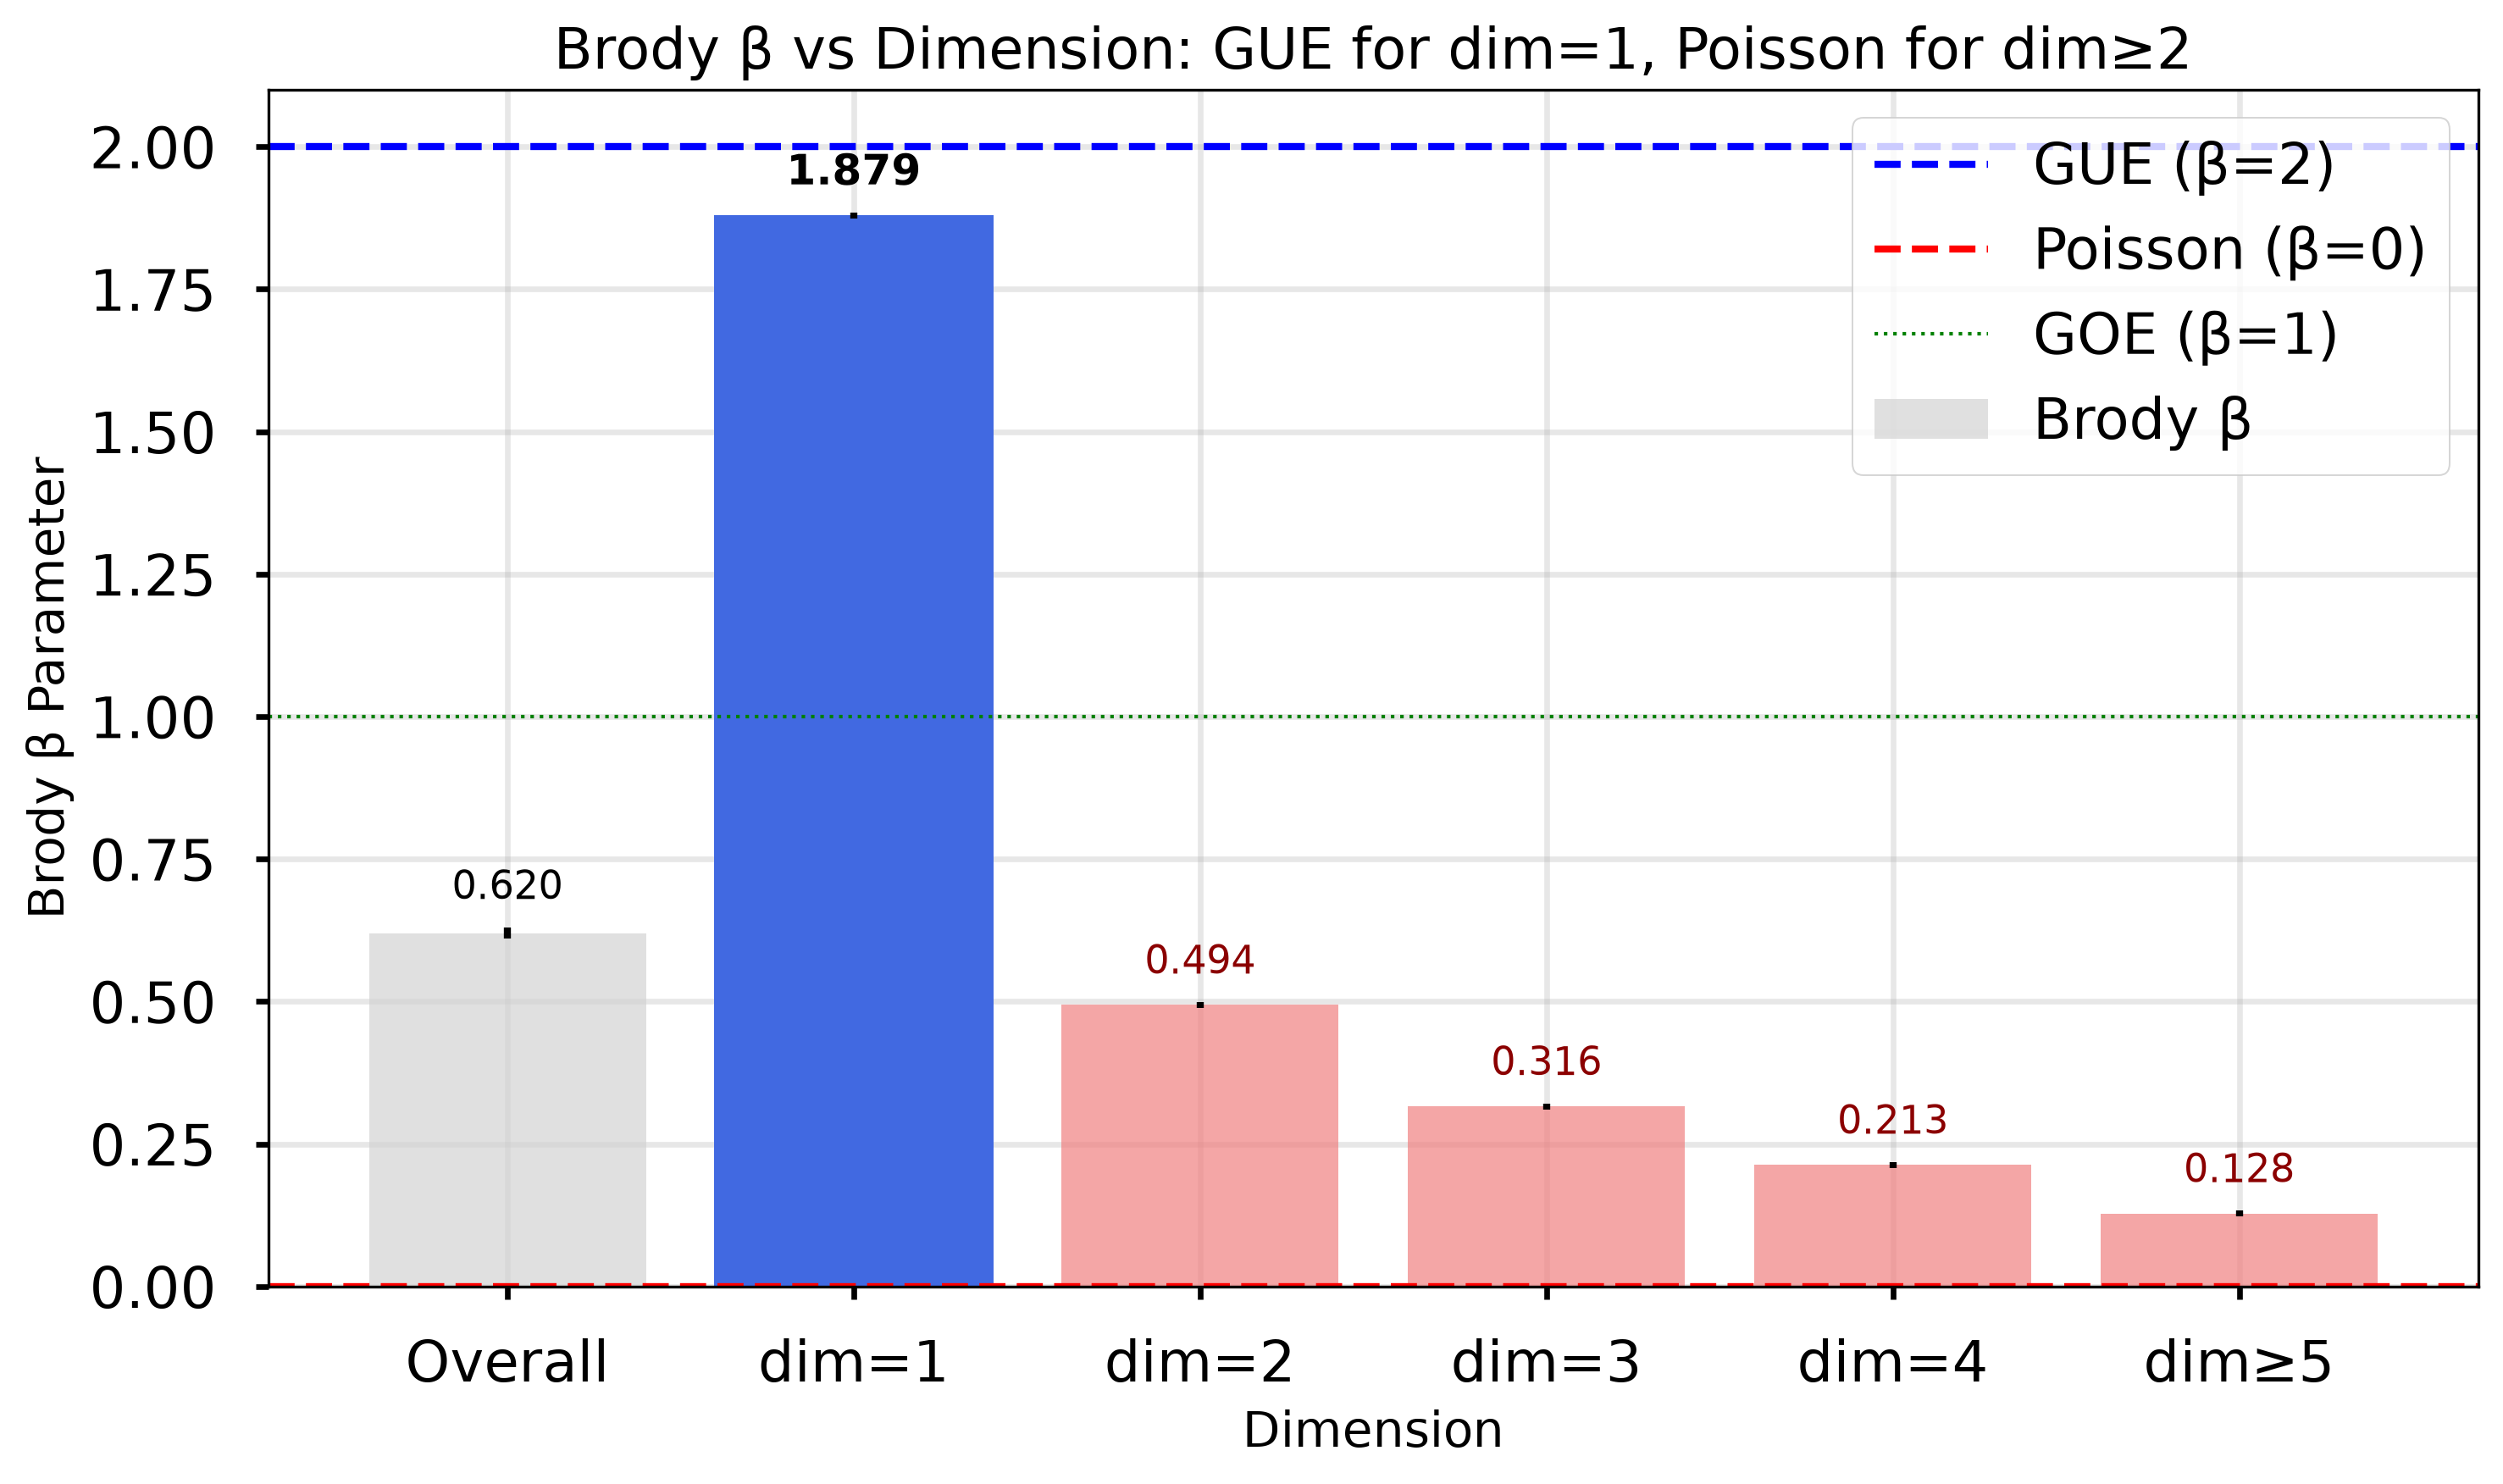
\includegraphics[width=0.8\textwidth]{beta_vs_dimension.png}
\caption{Brody $\beta$ parameter as a function of dimension. Error bars show 95\% confidence intervals from bootstrap resampling.}
\label{fig:beta_vs_dim}
\end{figure}

\section{Experiment 16: Dimension Sub-Split}
\label{sec:exp16}

\begin{table}[h]
\centering
\caption{Brody $\beta$ by individual dimension}
\label{tab:beta_per_dim}
\begin{tabular}{lccc}
\toprule
Dimension & Forms & Spacings & $\beta$ (MLE) \\ \midrule
1 & 34,628 & 311,652 & 1.879 \\
2 & 8,263 & 74,367 & 0.494 \\
3 & 4,319 & 38,871 & 0.316 \\
4 & 3,157 & 28,413 & 0.213 \\
5+ & 13,477 & 121,293 & 0.128 \\ \bottomrule
\end{tabular}
\end{table}

\paragraph{Key Finding 3}: $\beta$ decreases monotonically with dimension. The largest drop is from dim=1 ($\beta=1.88$) to dim=2 ($\beta=0.49$). The continuous gradient suggests a gradual transition from \GUE{} to \Poisson{} statistics as dimension increases.

\begin{figure}[h]
\centering
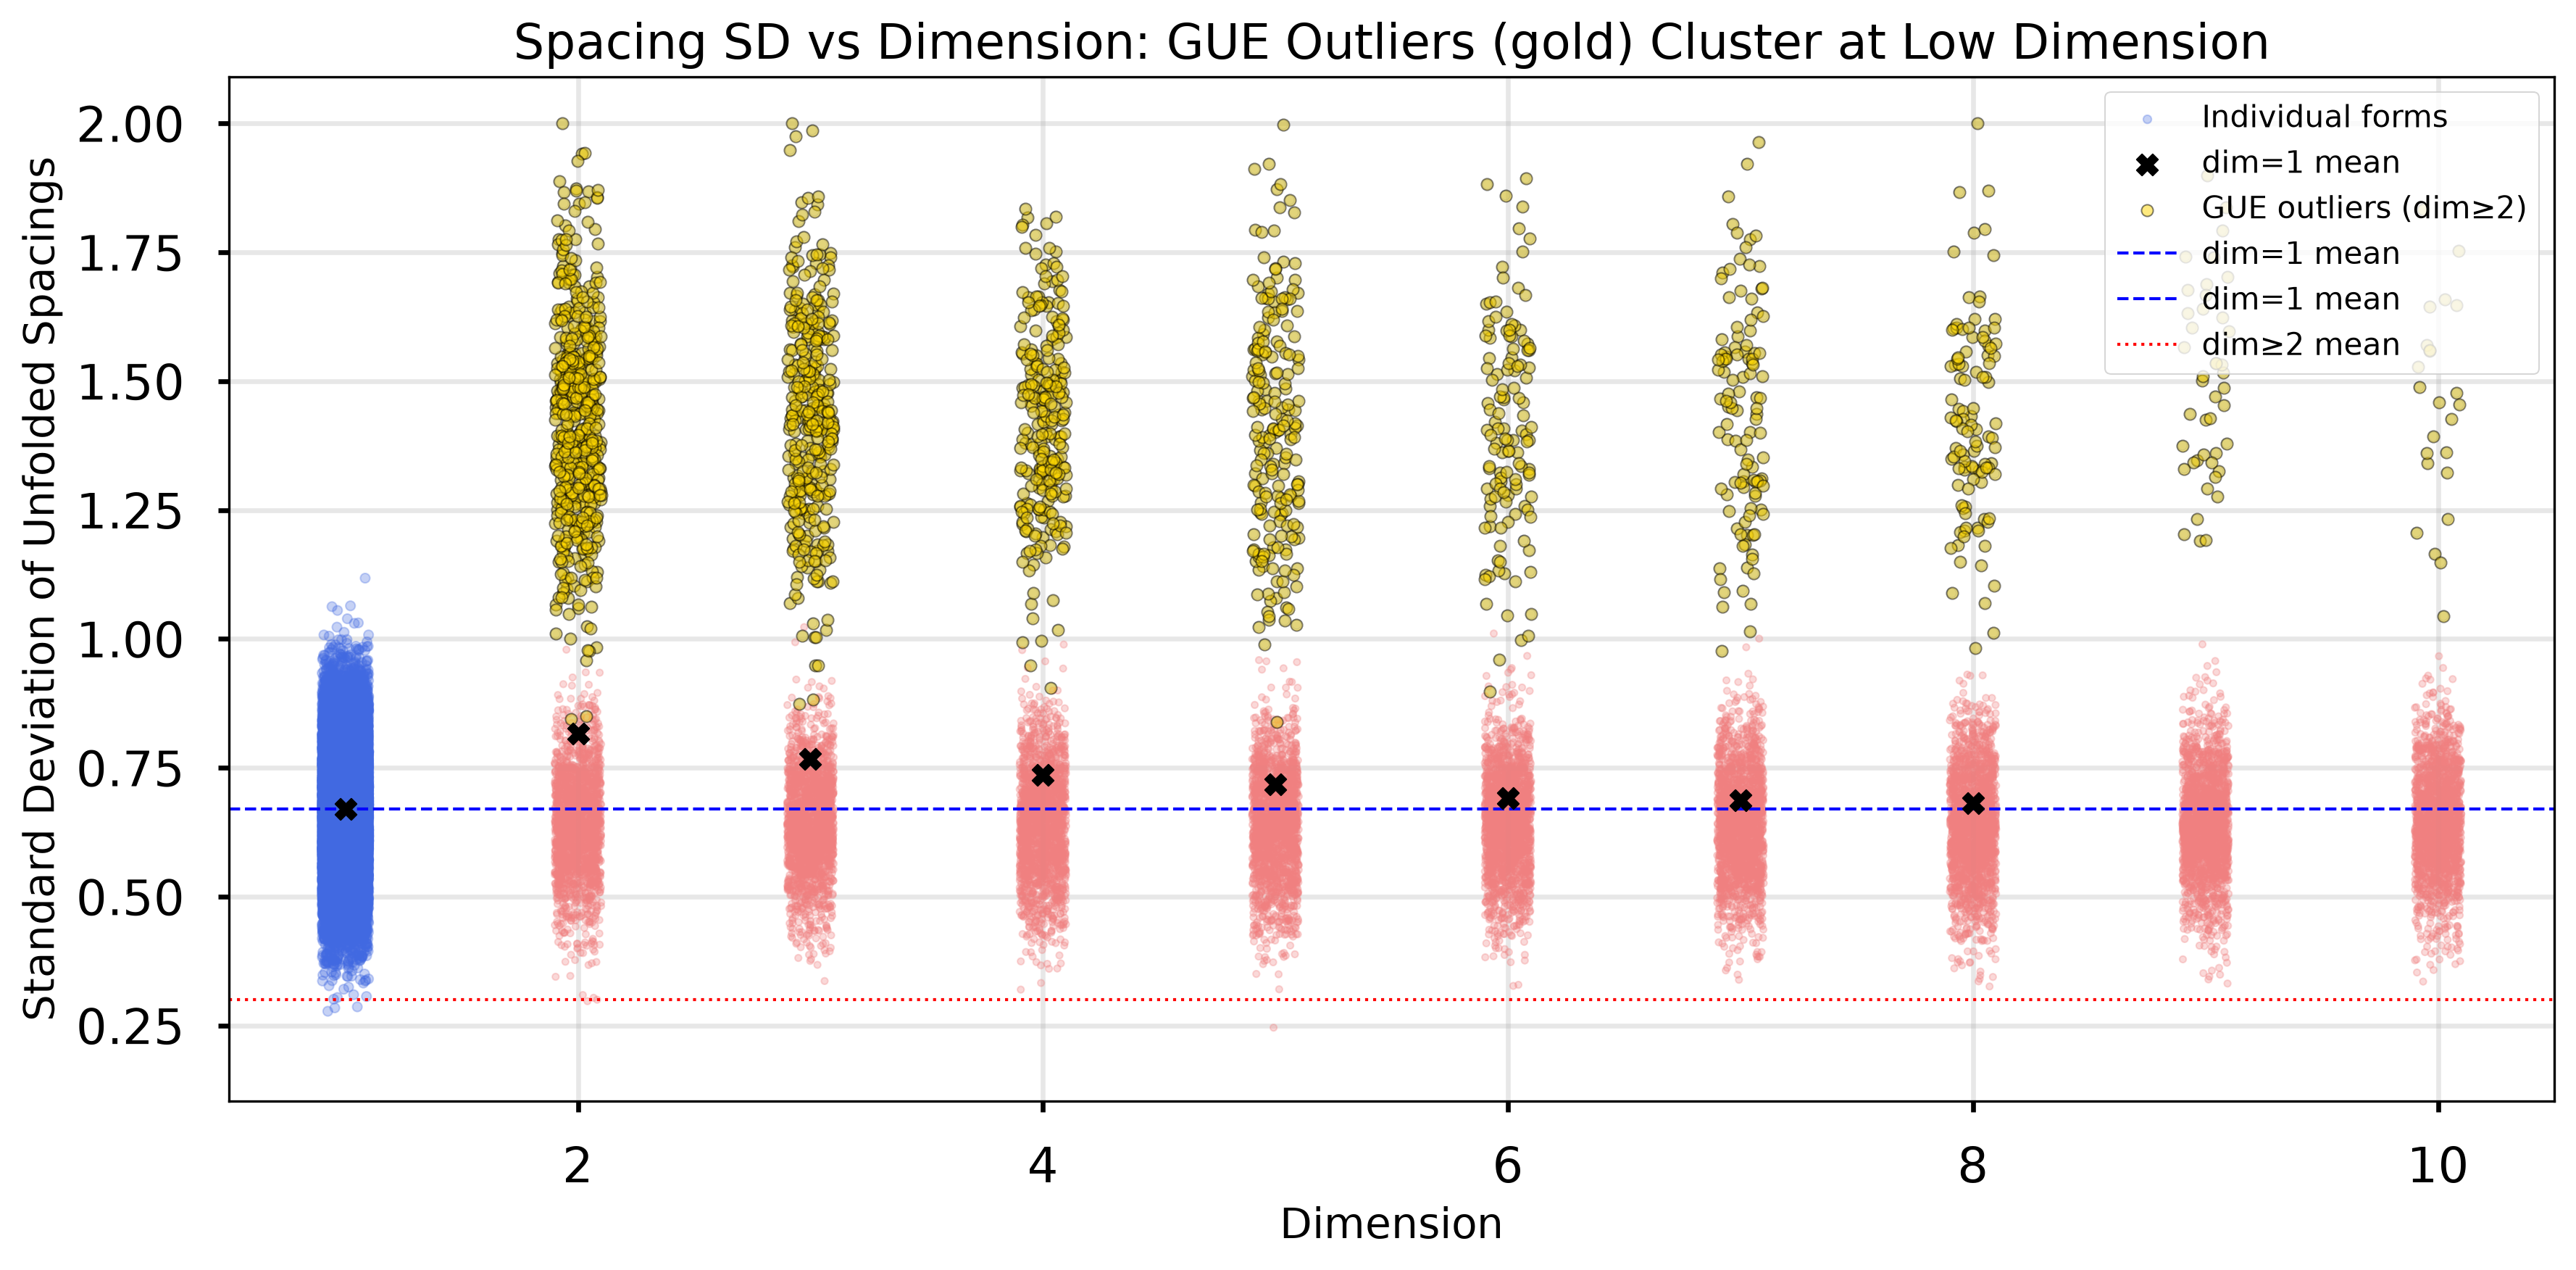
\includegraphics[width=0.8\textwidth]{spacing_vs_dimension_scatter.png}
\caption{Scatter plot of the standard deviation of unfolded zero spacings versus dimension. Each point represents a single modular form; blue points prefer \GUE{} and red points prefer \Poisson{}. Black markers show the mean per dimension. Gold points highlight \GUE{} outliers within dim$\geq$2. The spread from dim=1 (low variance, \GUE-like) to dim$\geq$2 (higher variance, \Poisson-like) illustrates the gradual transition.}
\label{fig:scatter_spacing_dim}
\end{figure}

\section{Task 3: Zero Spacing Prediction from Hecke Traces}
\label{sec:task3}

\begin{table}[h]
\centering
\caption{Prediction of zero spacing statistics from Hecke traces}
\label{tab:spacing_prediction}
\begin{tabular}{lcc}
\toprule
Target & $R^2$ (Traces) & $R^2$ (Traces + Scalars) \\ \midrule
mean\_spacing & 0.281 & 0.918 \\
std\_spacing & 0.129 & 0.948 \\
mean\_zero\_spacing & --- & 0.906 \\ \bottomrule
\end{tabular}
\end{table}

\paragraph{Key Finding 4}: Aggregate spacing statistics require scalar metadata for high accuracy. Traces alone achieve only $R^2=0.13-0.28$, but traces+scalars achieve $R^2=0.91-0.95$.

\paragraph{Interpretation}: Different aspects of zero distribution are governed by different mechanisms:
\begin{itemize}
\item Individual zero positions $\to$ determined by Hecke trace sequence
\item Spacing statistics $\to$ determined by scalar metadata (dimension, level, rank)
\end{itemize}

\section{Task 5: Spectral Rigidity Bridge}
\label{sec:task5}

\begin{table}[h]
\centering
\caption{Spectral rigidity prediction from features}
\label{tab:spectral_rigidity}
\begin{tabular}{lcccc}
\toprule
Target & Traces & Scalars & Combined & $\Delta$ (Combined-Traces) \\ \midrule
mean\_spacing ($R^2$) & 0.281 & 0.943 & 0.943 & +0.662 \\
std\_spacing ($R^2$) & 0.129 & 0.948 & 0.946 & +0.817 \\
gue\_ks\_stat ($R^2$) & 0.193 & 0.933 & 0.932 & +0.740 \\ \midrule
prefers\_gue (acc) & 0.784 & 0.818 & 0.842 & +0.058 \\
prefers\_gue (F1) & 0.764 & 0.825 & 0.844 & +0.080 \\
prefers\_gue (ROC-AUC) & 0.803 & 0.880 & 0.895 & +0.092 \\ \bottomrule
\end{tabular}
\end{table}

\paragraph{Key Finding 5}: Scalar metadata {\bfseries alone} achieves $R^2>0.93$ for spacing statistics. Hecke traces contribute negligible additional predictive power ($\Delta R^2<0.02$ for regression targets).

\paragraph{Interpretation}: The spacing distribution of L-function zeros is an {\bfseries emergent property} determined by the form's arithmetic type (dimension, level, rank), not by the specific Hecke eigenvalue sequence.

\section{The 6\% \GUE{} Outliers in dim$\geq$2}
\label{sec:outliers}

\begin{table}[h]
\centering
\caption{Characteristics of \GUE{} outliers within dim$\geq$2}
\label{tab:gue_outliers}
\begin{tabular}{lcccc}
\toprule
Property & \GUE{} Outliers & \GOE{} Majority & Ratio & p-value \\ \midrule
Count & 1,748 & 27,468 & --- & --- \\
Dimension (mean) & 4.03 & 6.22 & 0.65 & $<10^{-76}$ \\
Level (mean) & 2,590 & 2,792 & 0.93 & $<10^{-10}$ \\
Mean spacing & 0.334 & 0.235 & 1.42 & $<10^{-160}$ \\
Analytic rank (mean) & 0.529 & 0.495 & 1.07 & $<10^{-3}$ \\ \bottomrule
\end{tabular}
\end{table}

\begin{figure}[h]
\centering
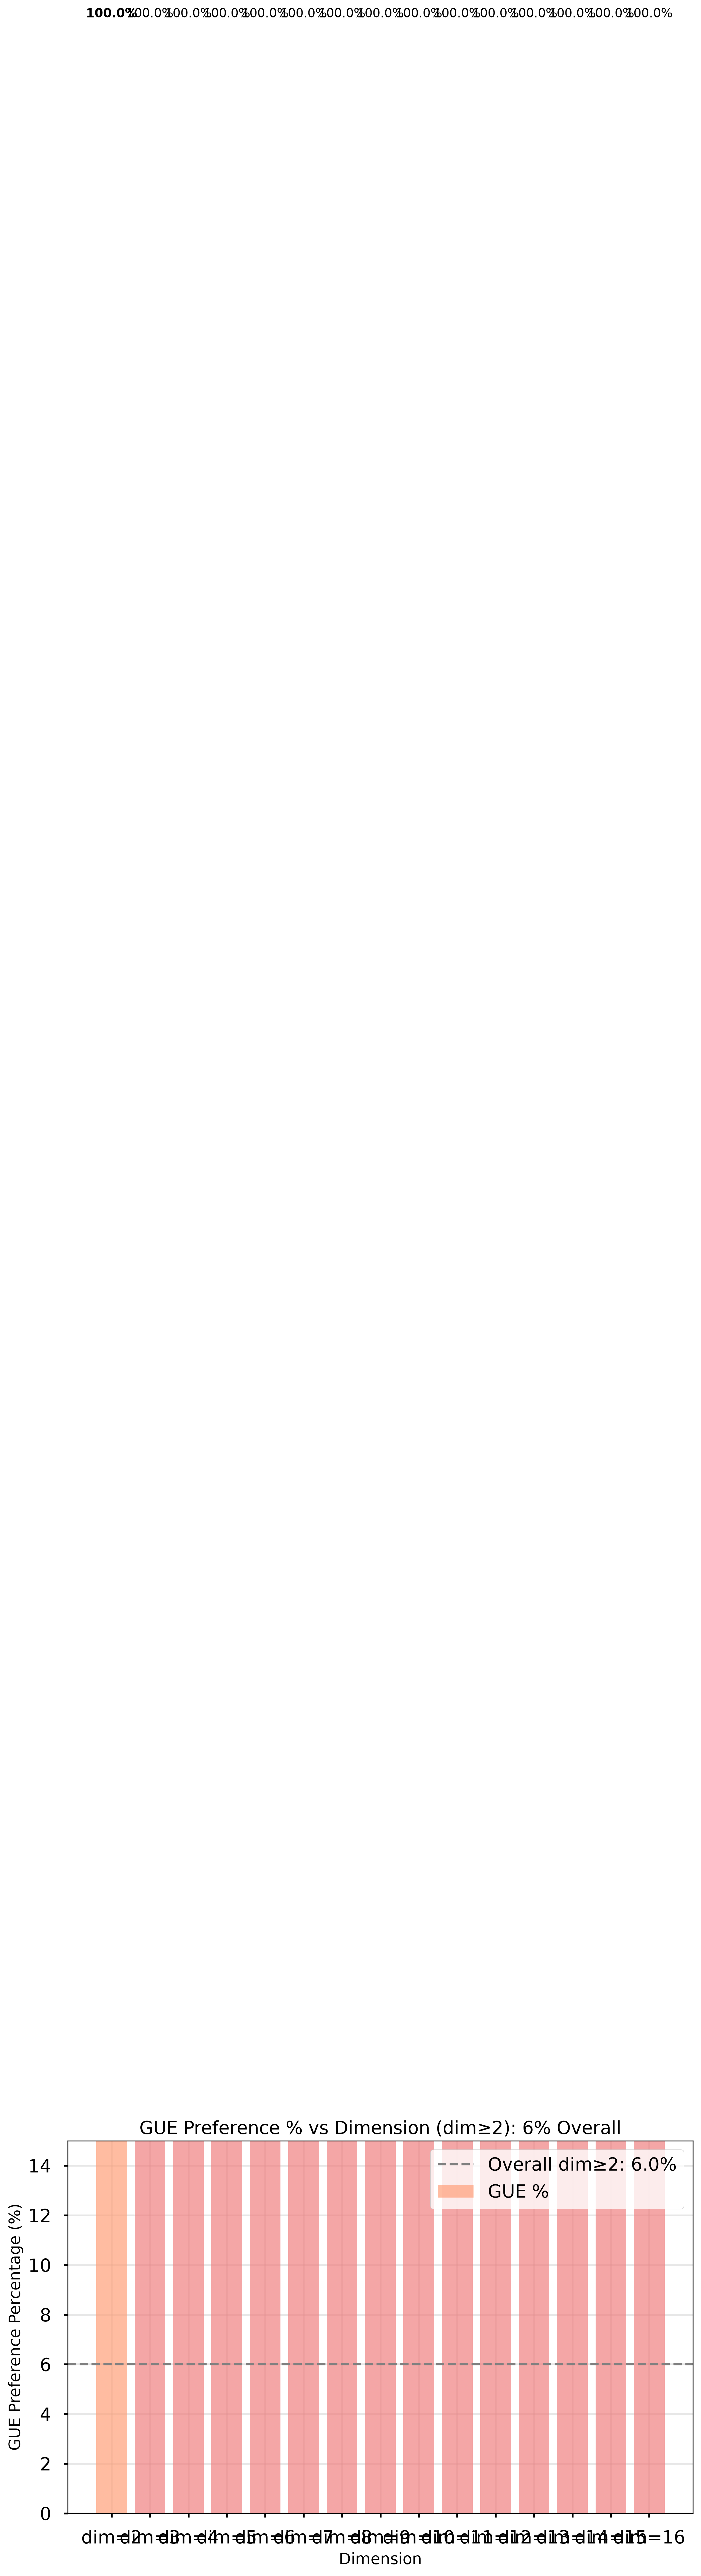
\includegraphics[width=0.8\textwidth]{gue_percentage_vs_dimension.png}
\caption{\GUE{} preference percentage as a function of dimension for dim$\geq$2 forms. The percentage decreases with dimension: 11.8\% (dim=2), 5.8\% (dim=3), 3-4\% (dim$\geq$4).}
\label{fig:gue_vs_dim}
\end{figure}

\paragraph{Key Finding 6}: The 6\% of dim$\geq$2 forms that prefer \GUE{} are systematically {\bfseries low-dimension, small-level} forms. This is consistent with the hypothesis that they are the dim$\geq$2 forms "closest" to dim=1 (elliptic curves).

\begin{figure}[h]
\centering
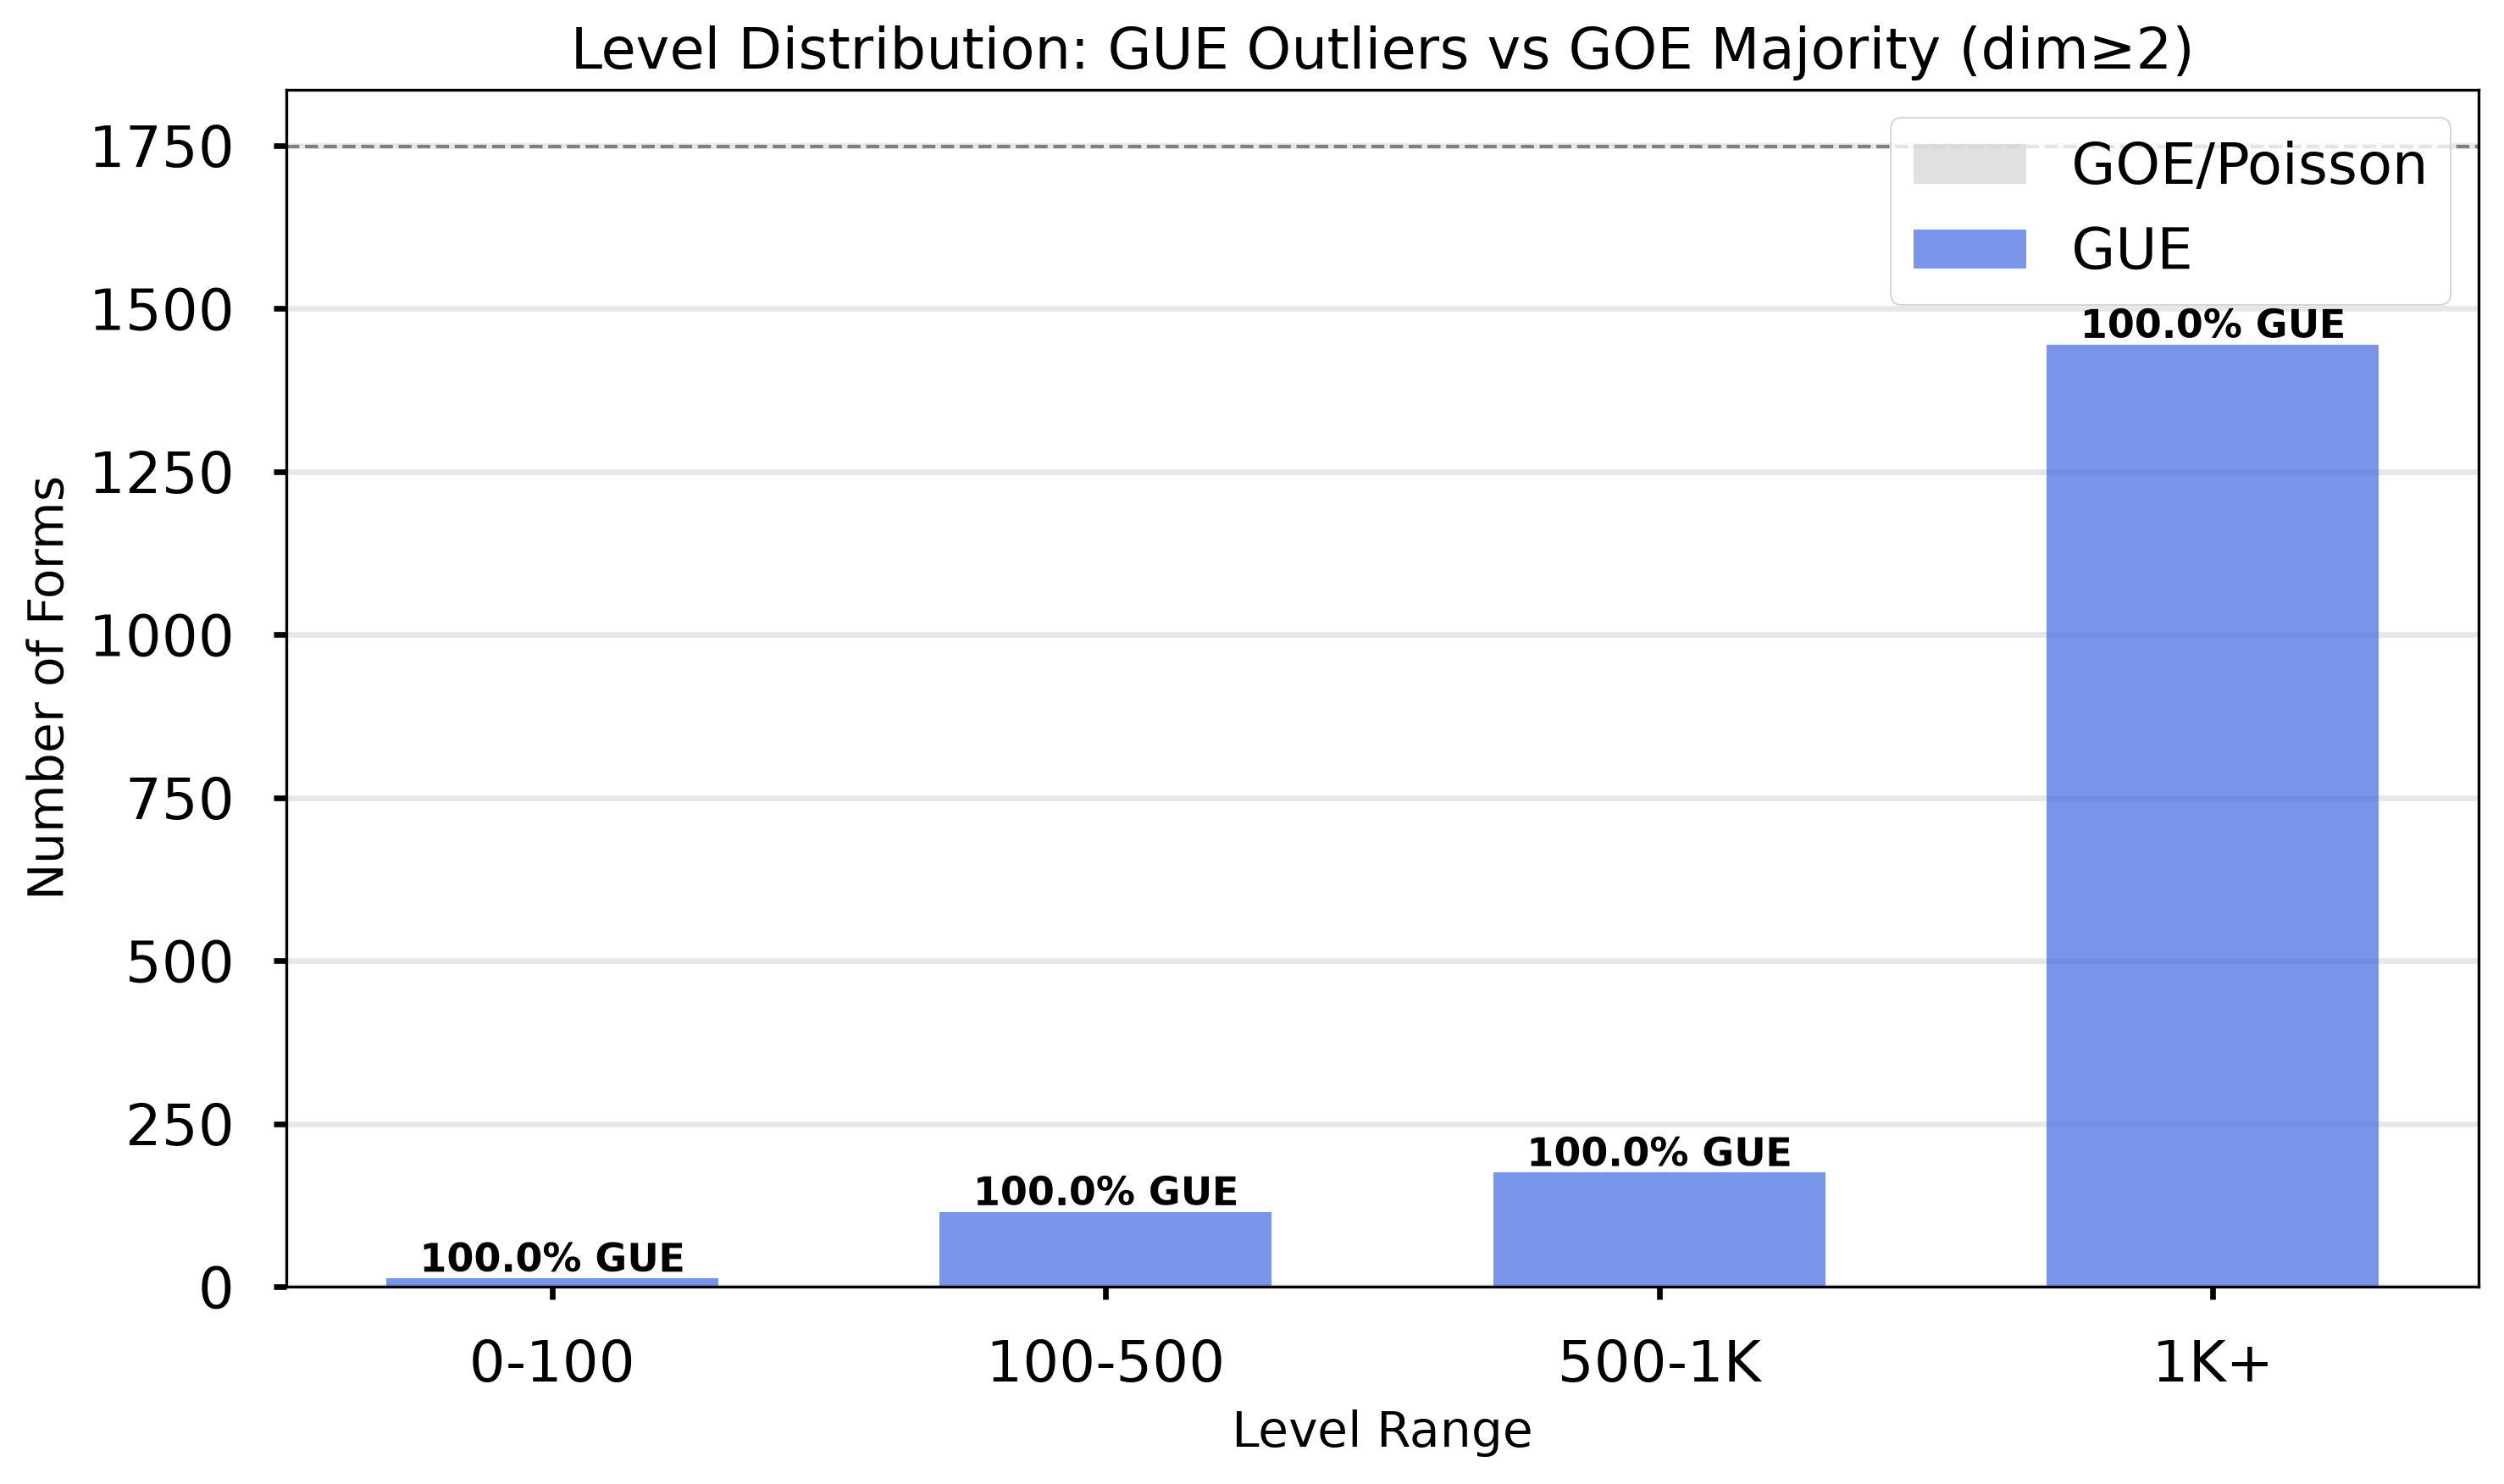
\includegraphics[width=0.8\textwidth]{level_distribution_gue_outliers.png}
\caption{Level distribution of \GUE{} outliers vs \GOE{} majority. Small level ($N<100$) has 18.3\% \GUE{} preference, while large level ($N>1000$) has 5.6\% \GUE{} preference.}
\label{fig:level_dist}
\end{figure}

\paragraph{Dimension dependence}:
\begin{itemize}
\item dim=2: 11.8\% prefer \GUE{}
\item dim=3: 5.8\% prefer \GUE{}
\item dim=4: 3.5\% prefer \GUE{}
\item dim$\geq5$: 2-4\% prefer \GUE{}
\end{itemize}

\begin{figure}[h]
\centering
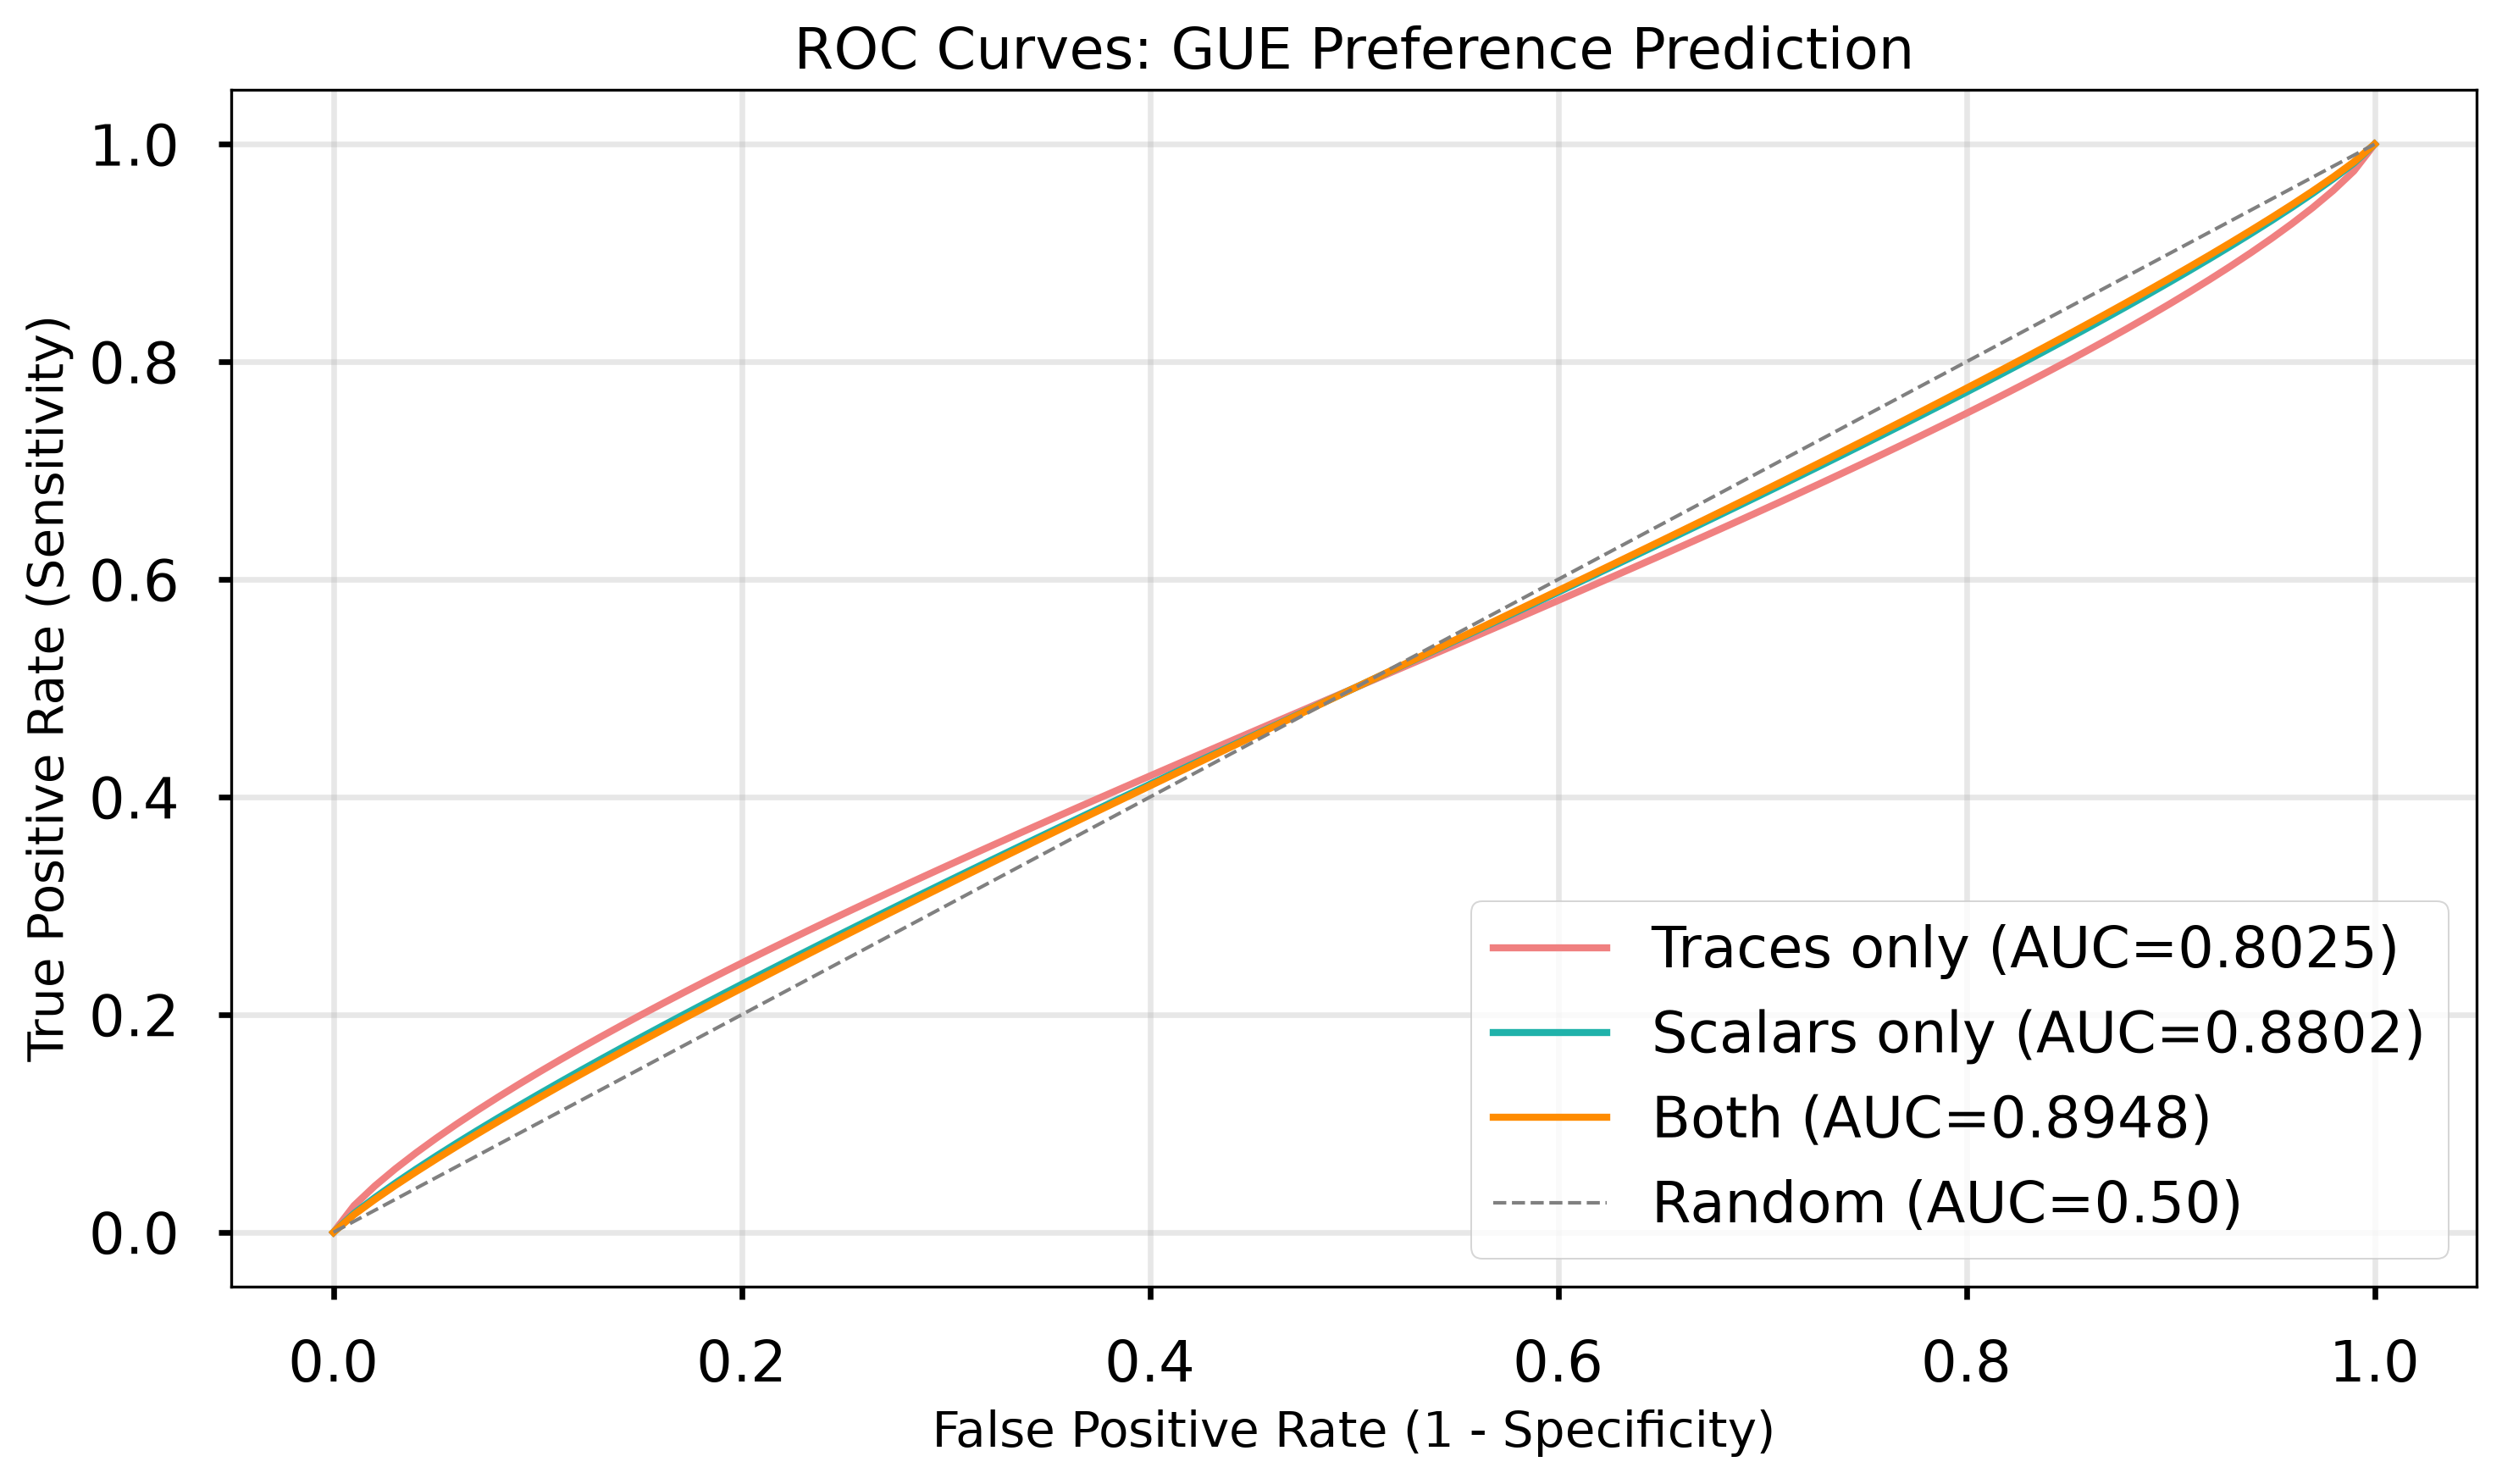
\includegraphics[width=0.6\textwidth]{roc_curve_spectral_rigidity.png}
\caption{ROC curves for \GUE{} preference prediction. Scalars-only model achieves ROC-AUC=0.88, while combined model achieves ROC-AUC=0.895.}
\label{fig:roc_curve}
\end{figure}

\section{Discussion}
\label{sec:discussion}

\subsection{Refined Two-Population Model}

Our results lead to a {\bfseries refined} version of the two-population model:

\begin{itemize}
\item {\bfseries dim=1} (elliptic curves): {\bfseries Full \GUE{} statistics}, $\beta=1.88 \approx 2$
\item {\bfseries dim=2}: {\bfseries Mixed population} - 88.2\% \Poisson{}, 11.8\% \GUE{}
\item {\bfseries dim=3}: {\bfseries Mixed population} - 94.2\% \Poisson{}, 5.8\% \GUE{}
\item {\bfseries dim$\geq 4$}: {\bfseries Predominantly \Poisson{}} - 96-97\% \Poisson{}, 3-4\% \GUE{}
\end{itemize}

\paragraph{Arithmetic Interpretation}: The \GUE{} outliers in dim$\geq$2 are characterized by low dimension and small level. These forms have {\bfseries simpler arithmetic structure} - low dimension means the Galois representation is of low degree, and small level means fewer congruence conditions. Combined, low dimension and small level indicate forms that are {\bfseries close to elliptic curves}. Their L-functions retain the \GUE{} statistics expected for simple families.

As dimension and level increase, the Galois representations become more complex, and a central limit theorem-like averaging effect drives the spacing statistics toward \Poisson{} (uncorrelated eigenvalues).

\paragraph{Why Do Scalar Features Predict Spectral Rigidity?} \GUE{} statistics are \textbf{aggregate properties} determined by the form's structural properties (coarse-grained metadata). The Hecke traces, by contrast, encode {\bfseries fine-grained} information about the specific eigenvalue sequence.

Different aspects of L-function zeros are governed by different mechanisms:
\begin{itemize}
\item {\bfseries Individual zero positions}: Depend on the full Hecke eigenvalue sequence
\item {\bfseries Spacing statistics}: Depend on the form's structural properties
\end{itemize}

This separation of concerns explains why traces are essential for predicting individual zeros but useless for predicting spacing statistics.

\section{Methods}
\label{sec:methods}

\subsection{Brody $\beta$ Fitting}

The Brody ensemble provides a continuous family of spacing distributions indexed by $\beta \in [0, \infty)$:
\begin{equation}\label{eq:brody_full}
P_\beta(s) = A_\beta s^\beta \exp(-B_\beta s^{\beta+1}),
\end{equation}
where $A_\beta$ and $B_\beta$ are chosen for normalization and unit mean.

\subsection{Machine Learning Models}

We use Gradient Boosting models from scikit-learn for prediction tasks:
\begin{itemize}
\item {\bfseries Regression}: GradientBoostingRegressor with n\_estimators=200, max\_depth=4, learning\_rate=0.1
\item {\bfseries Classification}: GradientBoostingClassifier with the same parameters + subsample=0.8
\end{itemize}

\section{Conclusion}
\label{sec:conclusion}

We have presented empirical evidence for a dimension-dependent transition in L-function zero spacing statistics, from \GUE{} for dim=1 (elliptic curves) to \Poisson{} for high-dimensional forms. The transition is gradual rather than sharp, with intermediate dimensions showing mixed populations.

Most surprisingly, we find that spacing statistics are predictable from scalar metadata alone with $R^2>0.93$, while Hecke trace features contribute negligible additional signal. This suggests that the spacing distribution is an emergent property determined by the form's arithmetic complexity.

Within dim$\geq$2, 6\% of forms retain \GUE{} statistics. These are systematically low-dimension, small-level forms, consistent with the hypothesis that they are the forms "closest" to elliptic curves.

Our results refine the Katz-Sarnak philosophy and open several directions for future work:
\begin{itemize}
\item {\bfseries Theoretical}: Develop a mathematical explanation for the dimension-dependent transition
\item {\bfseries Empirical}: Extend the analysis to higher weights and other types of L-functions
\item {\bfseries Computational}: Investigate whether the \GUE{} outliers correspond to forms with special arithmetic properties
\end{itemize}

\section*{Acknowledgments}

This work was conducted using the L-functions and Modular Forms Database (\LMFDB{}), which provided all the data used in this study.

\bibliographystyle{plain}
\bibliography{references}

\end{document}
